\section{Auswertung}
\label{sec:Auswertung}
\begin{figure}[ht]
    \centering
    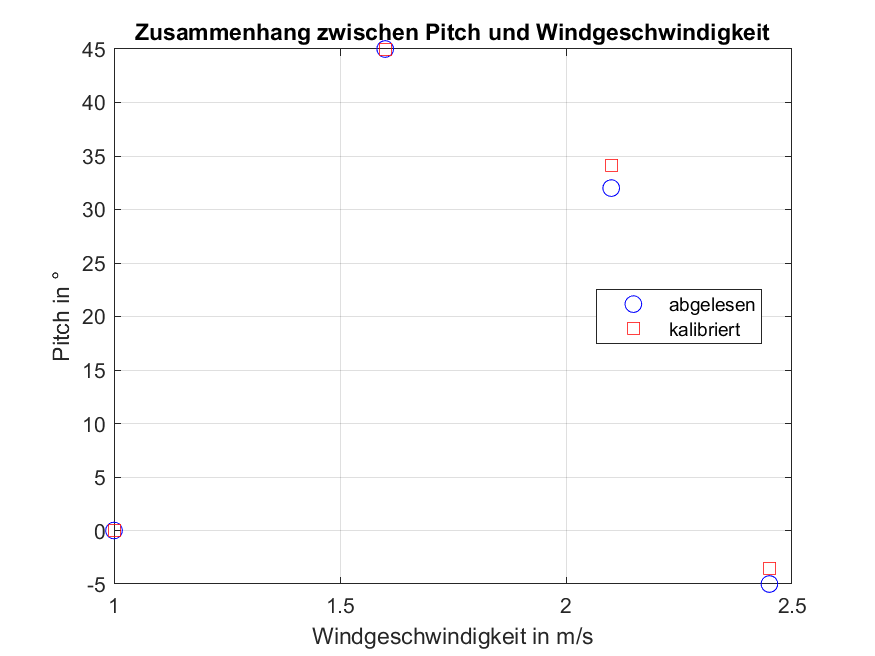
\includegraphics[width=\textwidth]{plot1}
    \caption{Bestrahlungsstärke je nach Entfernung aufgeteilt in links, mitte und rechts im Raum bei geschlossenem Fenster}
    \label{fig:plot1_28062023}
  \end{figure}
  \begin{figure}[ht]
    \centering
    \includegraphics[width=\textwidth]{plot2}
    \caption{Bestrahlungsstärke je nach Entfernung aufgeteilt in links, mitte und rechts im Raum bei offenem Fenster}
    \label{fig:plot2_28062023}
  \end{figure}
  \begin{figure}[H]
    \centering
    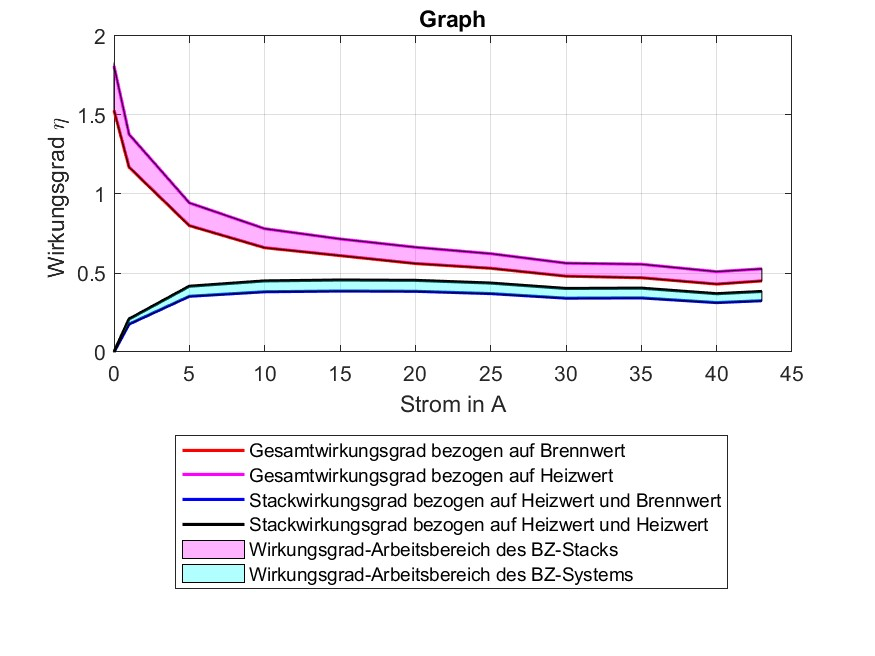
\includegraphics[width=\textwidth]{plot3}
    \caption{Bestrahlungsstärke je nach Entfernung aufgeteilt in links, mitte und rechts im Raum bei geschlossenem Fenster mit Kunstlicht}
    \label{fig:plot3_28062023}
  \end{figure}
  Nach Auswertung der vorliegenden Daten ergeben sich folgende Schlussfolgerungen.

Zunächst lässt sich feststellen, dass die Beleuchtungsstärke im betrachteten Raum von Fenster zu Tür hin abnimmt. Diese Abnahme zeigt sich in allen drei betrachteten Szenarien.

Des Weiteren zeigt sich, dass das Öffnen des Fensters, insbesondere wenn Prismenglas verwendet wird, zu einer signifikanten Steigerung der Beleuchtungsstärke führt. In der rechten Raumhälfte ist eine deutliche Zunahme zu beobachten, während in der linken Raumhälfte eine moderate Steigerung festzustellen ist.

Die Verwendung von künstlichem Licht trägt dazu bei, die Beleuchtungsverhältnisse im Raum zu stabilisieren. Allerdings führt dies auch zu erhöhten Beleuchtungsverhältnissen in der Nähe des Fensters. Um den Energieverbrauch zu senken und eine ausgewogenere Beleuchtungsstärke zwischen künstlichem Licht und Tageslicht zu erzielen, könnte eine Dimmung der Leuchten im Fensterbereich in Betracht gezogen werden.

Abschließend ist anzumerken, dass Tageslichtquotienten üblicherweise in Arbeitsbereichen bestimmt werden. Diese Quoten sollten idealerweise zwischen 1\% und 10\% liegen, um eine angemessene Beleuchtung für die durchzuführenden Arbeiten zu gewährleisten.